\documentclass[a4paper,12pt]{article}
\usepackage[utf8]{inputenc}
\usepackage{geometry}
\usepackage{graphicx}
\usepackage{listings}
\usepackage{xcolor}
\usepackage{tikz}
\usepackage{float} 
\usetikzlibrary{shapes, arrows, positioning, fit, calc}

% Config
\definecolor{codegreen}{rgb}{0,0.6,0}
\definecolor{codegray}{rgb}{0.5,0.5,0.5}
\definecolor{backcolour}{rgb}{0.95,0.95,0.92}

\lstdefinestyle{mystyle}{
    backgroundcolor=\color{backcolour},   
    commentstyle=\color{codegreen},
    basicstyle=\ttfamily\footnotesize,
    breakatwhitespace=false,         
    breaklines=true,                 
    captionpos=b,                    
    keepspaces=true,                 
    numbers=left,                    
    numbersep=5pt,                  
    showspaces=false,                
    showtabs=false,                  
    tabsize=2,
    frame=single
}
\lstset{style=mystyle}

\title{Practical Work 4: Word Count with MapReduce}
\author{Le Quy Ton \\ 23BI14425}
\date{\today}

\begin{document}

\maketitle

\section{Introduction}
The objective of this practical work is to implement the classic "Word Count" problem using the MapReduce programming model. We aim to understand the flow of data processing including Mapping, Shuffling, and Reducing.

\section{Implementation Choice}
We chose a \textbf{Python-based Streaming approach} combined with Linux standard utilities.
\begin{itemize}
    \item \textbf{Why Python?} It allows for rapid development of the Mapper and Reducer logic with clean syntax for string manipulation.
    \item \textbf{Why Linux Pipes?} Following the "Invent yourself" guideline, we utilized the Unix philosophy. Instead of setting up a heavy Hadoop cluster, we simulate the distributed nature using the pipeline:
    \begin{center}
        \texttt{cat input.txt | ./mapper.py | sort | ./reducer.py}
    \end{center}
    This effectively demonstrates the MapReduce architecture where \texttt{sort} handles the crucial "Shuffle and Sort" phase.
\end{itemize}

\section{System Design and Operation}

\subsection{Mapper Logic}
The Mapper reads text line by line. It tokenizes the text into words and emits a key-value pair for each word: $<word, 1>$.

\subsection{Reducer Logic}
The Reducer receives sorted input (grouped by keys). It iterates through the lines, summing up the counts for identical consecutive keys. When a new key appears, it outputs the total for the previous key.

\subsection{Process Visualization}
Figure \ref{fig:mapreduce} illustrates how our code processes the input "three witches watch three".

\begin{figure}[H]
    \centering
    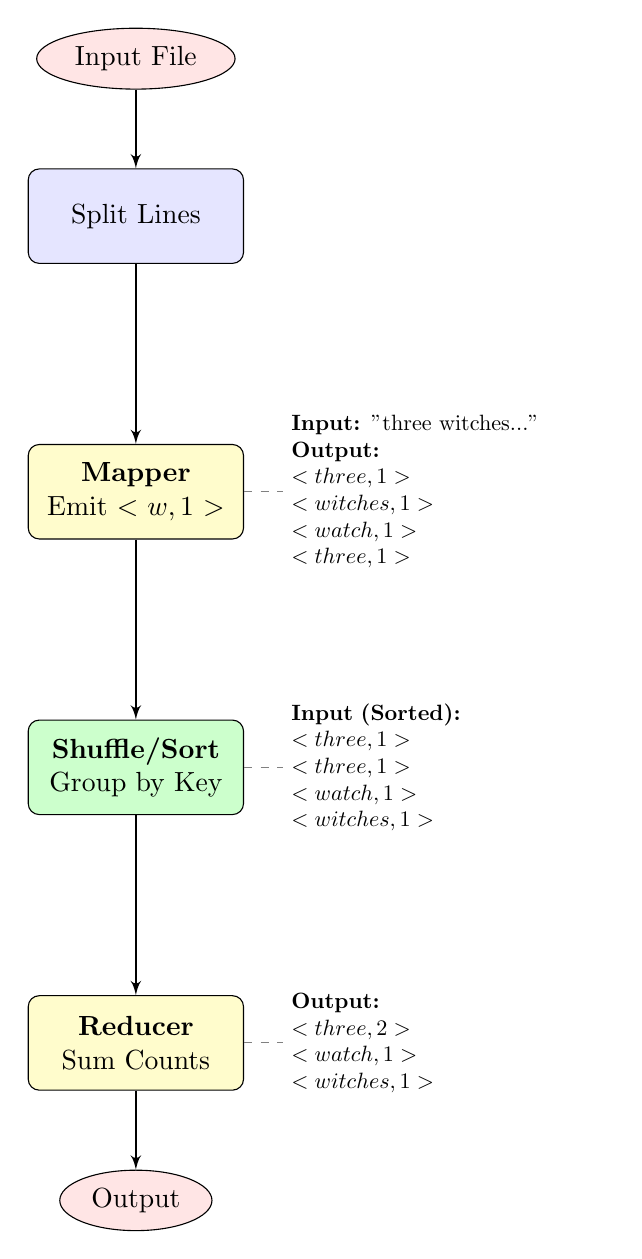
\begin{tikzpicture}[node distance=3.5cm, auto,
        block/.style={rectangle, draw, fill=blue!10, text width=2.5cm, align=center, rounded corners, minimum height=1.2cm},
        cloud/.style={draw, ellipse, fill=red!10, node distance=3.5cm, minimum height=2em},
        line/.style={draw, -latex', thick}]


        \node [cloud] (input) {Input File};
        \node [block, below of=input, node distance=2cm] (split) {Split Lines};
        \node [block, below of=split, fill=yellow!20] (map) {\textbf{Mapper}\\Emit $<w, 1>$};
        \node [block, below of=map, fill=green!20] (shuffle) {\textbf{Shuffle/Sort}\\Group by Key};
        \node [block, below of=shuffle, fill=yellow!20] (reduce) {\textbf{Reducer}\\Sum Counts};
        \node [cloud, below of=reduce, node distance=2cm] (output) {Output};

        \node [right=0.5cm of map, text width=5cm, scale=0.8, align=left] (mapdata) {
            \textbf{Input:} "three witches..."\\
            \textbf{Output:}\\
            $<three, 1>$\\
            $<witches, 1>$\\
            $<watch, 1>$\\
            $<three, 1>$
        };
        
        \node [right=0.5cm of shuffle, text width=5cm, scale=0.8, align=left] (shuffledata) {
            \textbf{Input (Sorted):}\\
            $<three, 1>$\\
            $<three, 1>$\\
            $<watch, 1>$\\
            $<witches, 1>$
        };

        \node [right=0.5cm of reduce, text width=5cm, scale=0.8, align=left] (reducedata) {
            \textbf{Output:}\\
            $<three, 2>$\\
            $<watch, 1>$\\
            $<witches, 1>$
        };

        % Paths
        \path [line] (input) -- (split);
        \path [line] (split) -- (map);
        \path [line] (map) -- (shuffle);
        \path [line] (shuffle) -- (reduce);
        \path [line] (reduce) -- (output);
        
        % Drawing lines to annotations
        \draw [dashed, gray] (map) -- (mapdata);
        \draw [dashed, gray] (shuffle) -- (shuffledata);
        \draw [dashed, gray] (reduce) -- (reducedata);

    \end{tikzpicture}
    \caption{Workflow of the implemented Word Count MapReduce}
    \label{fig:mapreduce}
\end{figure}

\section{Execution and Results}
We verified the implementation by running it on a Linux environment (Debian). We created a dummy input file \texttt{input.txt} containing repeated words and executed the pipeline.

Figure \ref{fig:execution} shows the terminal output, confirming that the system correctly counts the occurrences of each word (e.g., "bon" appears 4 times, "ba" appears 2 times).

\begin{figure}[H]
    \centering
    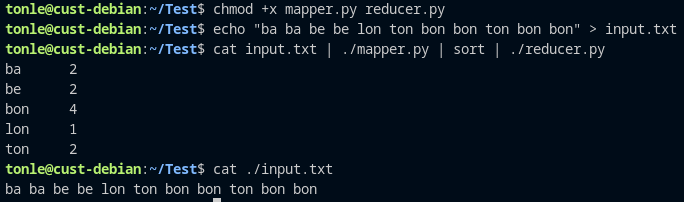
\includegraphics[width=0.95\linewidth]{image1.png}
    \caption{Successful execution of MapReduce Word Count}
    \label{fig:execution}
\end{figure}

\section{Code Implementation}

\subsection{Mapper (mapper.py)}
\begin{lstlisting}[language=Python]
import sys
for line in sys.stdin:
    words = line.strip().split()
    for word in words:
        print(f"{word}\t1")
\end{lstlisting}

\subsection{Reducer (reducer.py)}
\begin{lstlisting}[language=Python]
import sys
curr_word = None
curr_count = 0

for line in sys.stdin:
    word, count = line.strip().split('\t', 1)
    count = int(count)
    if curr_word == word:
        curr_count += count
    else:
        if curr_word:
            print(f"{curr_word}\t{curr_count}")
        curr_word = word
        curr_count = count
if curr_word:
    print(f"{curr_word}\t{curr_count}")
\end{lstlisting}

\section{Conclusion}
In this practical work, we successfully implemented a Word Count application using the MapReduce paradigm without relying on complex frameworks like Hadoop or Spark. By utilizing Python for logic processing and Linux pipes for data streaming and sorting, we gained a clear understanding of the underlying mechanics of MapReduce.

The experiment demonstrated that the core efficiency of MapReduce lies in the "Shuffle and Sort" phase, which groups related data together, allowing the Reducer to process data sequentially. This lightweight implementation serves as a strong foundation for understanding how large-scale distributed systems process massive datasets.

\end{document}
